\chapter{The CMS Tracker Upgrade}\label{chapter:tk-upgrade}
 
\section{The High-Luminosity Large Hadron Collider} \label{sec:hl-lhc}
The High-Luminosity Large Hadron Collider (HL-HLC) upgrade is expected to be installed during Long Shutdown 3 (2023-2025), with the instantaneous luminosity of the LHC increasing up to $5-7.5 \times {10}^{34}$\percms, corresponding to an average number of proton-proton interactions per 40\MHz bunch crossing of 140 to 200, and a total integrated luminosity of 3000\fbinv to the ATLAS and CMS experiments.

Increasing the LHC's instantaneous luminosity is motivated by the need to replace the inner triplet quadrupole magnets which focus the beams at the ATLAS and CMS collision regions, that are expected to be near life expired due to radiation exposure by 2023~\cite{hl-lhc-prelim-design-report,CMSCollaboration:2015zni}.
This increase in instantaneous luminosity will provide the experiments the ability to overcome the diminishing statistical gains that occur the longer an experiment is operated for at constant luminosity, and so enable greater precision SM and Higgs measurements, searches for rare processes and their potential deviations from the SM, and the discovery reach for multi-\TeV massive particles.

The instantaneous luminosity of the machine and the beam parameters are related by: the number of bunches $n_{b}$, the number of protons per bunch $N^{2}_{p}$, the beam beta value (focal length) at the collision point $\beta^{*}$, and a crossing angle dependent luminosity geometrical reduction factor $R$,

\begin{equation}
L \propto \frac{n_{b}N^{2}_{p}}{\beta^{*}} R \\
\label{eq:machineLumi}
\end{equation}

As it is not practical to increase the number of proton bunches due to the resultant heat loads induced by electron clouds, the increase in the machine's luminosity will be achieved by increasing the number of protons per bunch and by  reducing $\beta^{*}$.
Replacing Linac2 with the new Linear accelerator 4 (Linac4) during the Long Shutdown 2 (2019-2020) will allow for the number of protons per bunch to be increased by a factor of two compared to the nominal LHC design (and to increase the injection energy by a factor of three)~\cite{linac4}.
The new more radiation tolerant quadrupole magnets to be installed during LS3 will provide the larger magnetic field strength and aperture required to provide the lower $\beta^{*}$ required for increasing the instantaneous luminosity. 

\section{The Phase-II Outer Tracker Upgrade}\label{sec:tk-upgrade}

To meet the significant challenges of, and exploit, the increased instantaneous luminosity environment of the HL-LHC, the CMS detector's ``Phase-II Upgrade'' during the LS3 will deliver the required improved radiation hardness for the increase in radiation and to manage the high \PU HL-LHC environment with greater detector granularity to reduce occupancy, and enhanced bandwidth and triggering capabilities to avoid compromising physics potential~\cite{CMSCollaboration:2015zni,P2TrackerTDR}.

The Phase-II upgrade will see both the entire silicon tracking detector being replaced with one comprised of a pixel Inner Tracker and pixel and strip Outer Tracker which have:
\begin{itemize}
\item \bf{improved radiation hardness} - being able to withstand the increased fluence of the HL-LHC (up to $2.3\times10^{16} n_{eq}/cm^{2}$ for the innermost layers)and operate efficiently up to the targeted luminosity of 3000\fbinv, with a margin of $\approx50\%$ to accommodate the target being exceeded and the uncertainties in the anticipated radiation exposure.
\item \bf{increased sensor granularity} - so that the channel occupancy is kept at or below the per cent (per mille) level for the Outer (Inner) Tracker, allowing for a high track reconstruction efficiency and a low misidentification rate under the increased \PU conditions. This will also enable improved track separation in dense environments, such as high \pT jets, compared to the current pixel detector and fully exploit the vast volume of data produced.
\item \bf{reduced material in the tracking volume} - the current tracker's performance is significantly impacted by the amount of material present, as are the calorimeters and overall performance of CMS.
Significant reducing the tracker's material budget will greatly enhance CMS' performance at the HL-LHC.
\item \bf{robust pattern recognition} - enabling fast and efficient track finding, which is especially important for the HLT, in the high \PU environment.
\item \bf{level-1 trigger contributions} - it has been shown that the L1 trigger performance will deteriorate in the high luminosity environment from both the rate increase and the reduced efficiencies of the L1 selection algorithms.
As raising the upgraded calorimeters' and muon chambers' trigger thresholds would have minimal impact on the rate, and 	would negatively impact sensitivity to low mass searches and measurements, the L1 bandwidth and latency will be increased (from 100\kHz to 750\kHz and from $3.2\mus$ to $12.5\mus$ respectively) and tracking information will be included in the L1 decision process to preserve and improve trigger performance.
\item \bf{extended tracking acceptance} - the overall physics capabilities of the CMS experiment would greatly benefit from extended coverage of the tracker and calorimeters up to $|\eta| = 4$ in the forward region.
\end{itemize}

With the above requirements in mind, the pixel Inner Tracker is designed to cover up to $|\eta| = 4$ with $100-150\mum$ thick planar silicon pixel sensors, measuring either $25\times100\mum^{2}$ or $50\times50\mum^{2}$\footnote{This is a reduction of a factor of $\approx 6$ compared to the Phase-0 and Phase-I pixel detectors}, which provide the low (per mille) occupancy and track separation with the negligible inefficiencies required in the harsh radiation environment.
Akin to the previous pixel detectors, the Phase-II pixel is also designed for easy installation and removal to facilitate the replacement of degraded parts.
Further discussion of the Inner Tracker is detailed in the Phase-II Technical Design Report~\cite{P2TrackerTDR}.

As tracking information is required to make L1 decisions at the HL-LHC, the design of the Outer Tracker has been driven by the need to provide tracking information to the L1 trigger.
Given the implications for reading out every hit for the L1 trigger at the LHC bunch crossing rate of 40\MHz, a novel design of a pair of closely spaced silicon sensors, capable of rejecting hits generated by low \pT particles, has been proposed, where the ``\pT modules''~\cite{jjonespixel,markthesis} discriminate on charged particle \pT based on the local bend of the track within the magnetic field, as shown in Fig.~\ref{fig:stubs}.
Pairs of clusters which are consistent with a track \pT above a configurable threshold (typically 2-3\GeV) will be correlated on-detector, and the resultant \emph{stubs} transferred to the L1 trigger, providing an effective data rate reduction of approximately a factor of 10~\cite{mpessimperf,2dptmoduleconcept}.

\begin{figure}[!t]
\centering
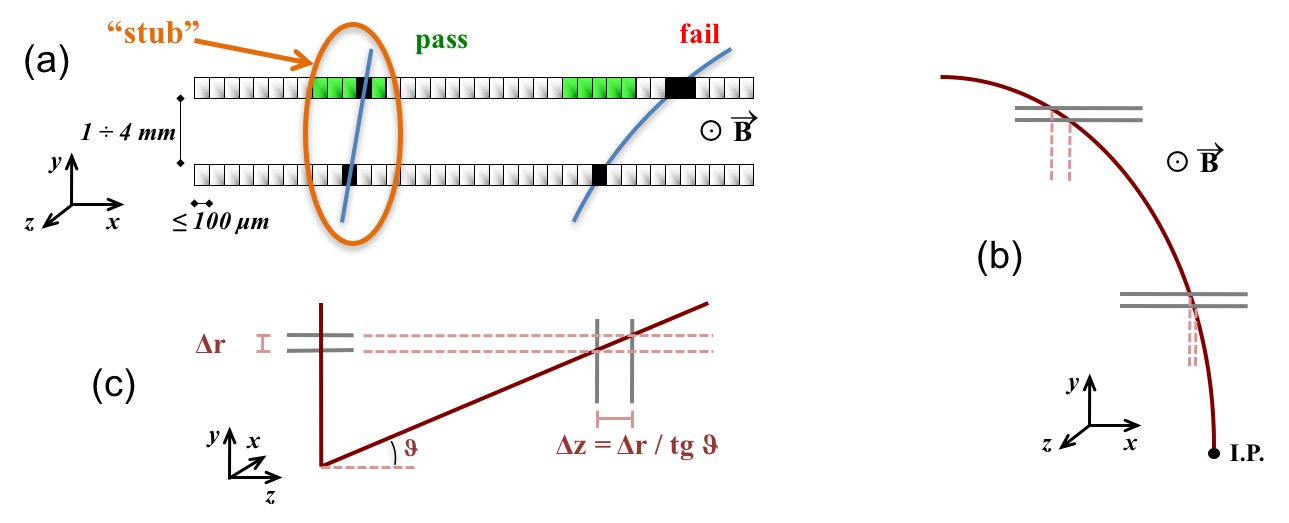
\includegraphics[width=5in]{figs/tk-upgrade/pTsketches.png}
% where an .eps filename suffix will be assumed under latex,
% and a .pdf suffix will be assumed for pdflatex; or what has been declared
% via \DeclareGraphicsExtensions.
\caption{Cluster matching in $p_\mathrm{T}$-modules~\cite{P2TrackerTDR}. (a) Correlating closely spaced clusters between two sensor layers, separated by a few mm, allows discrimination of transverse momentum based on the particle bend in the CMS magnetic field, assuming that the particle originated at the beam-line. (b) The same transverse momentum corresponds to a larger distance between signals for a given sensor spacing. (c) A larger spacing is needed in the endcap disks to achieve the same discrimination. Only tracks with \pT $> 2-3$\GeVc are transferred off-detector.
}
\label{fig:stubs}
\end{figure}

Two \pT modules are being developed for the Outer Tracker upgrade: 2S \emph{strip-strip} modules and PS \emph{pixel-strip} modules, both shown in Fig.~\ref{fig:2Spsmodules}.
The 2S~modules, are designed to be used at radii $r>60$\cm from the beam line, where the hit occupancies are lower and each sensor has an active area of 0.05\cm~$\times$~9.14\cm.
Both 2S~module strip layers have a pitch of 90\mum in the transverse plane, $r$-$\varphi$, and a strip length of 5.03\cm along the direction of the beam axis, $z$.
Each PS~module sensor layer has an active area of 4.69\cm~$\times$~9.60\cm, will be used at radii $20<r<60$\cm where the occupancies are highest.
The upper PS~module layer consist of an upper silicon strip sensor, and the lower a silicon pixel sensor, both with a pitch of 100\mum in $r$-$\varphi$, and a strip length in $z$ of 2.35\cm for the strips and 1.47\mm for the pixels.
The finer granularity provided by the pixel layer affords better resolution along the $z$ axis, which is crucial for vertex identification in the high \PU environment of the HL-LHC.
Further details on the two \pT modules can be found in~\cite{CMS_Upgrade_TP,P2TrackerTDR}.
 
\begin{figure}[tp]
\centering
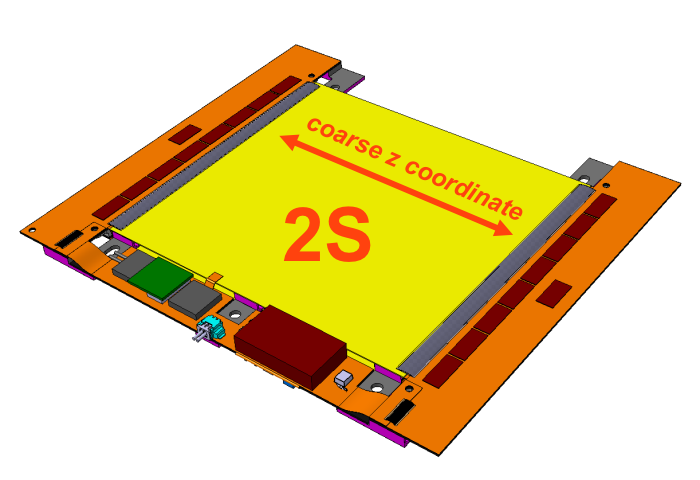
\includegraphics[width=0.55\textwidth,trim={0truecm 0truecm 0truecm 1truecm},clip]{figs/tk-upgrade/2S_assembled.png}
\hfill
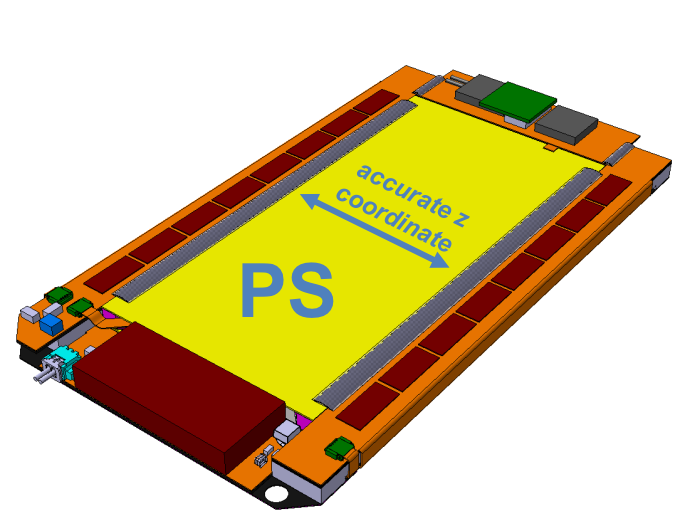
\includegraphics[width=0.44\textwidth,trim={0truecm 0truecm 0truecm 1truecm},clip]{figs/tk-upgrade/PS_assembled.png}
% where an .eps filename suffix will be assumed under latex,
% and a .pdf suffix will be assumed for pdflatex; or what has been declared
% via \DeclareGraphicsExtensions.
\caption{The 2S module (left) and PS module (right), described in the text~\cite{P2TrackerTDR}.}
\label{fig:2Spsmodules}
\end{figure}

The current proposed layout of the Phase-II Outer Tracker, referred to as the \emph{tilted barrel} geometry, is depicted in the upper diagram in Fig.~\ref{fig:trackerlayout}, illustrating the PS and 2S module positions in the six barrel layers and the five endcap disks either side of the barrel.
Only modules located at $|\eta| < 2.4$ will be configured to send stub data off-detector.
The geometry's name is inspired by modules in the three innermost barrel layers being tilted so that their normals point towards the interaction region.
This layout was adopted as it not only improves stub-finding efficiency for tracks with large incident angles but also reduces the overall cost of the system~\cite{P2TrackerTDR}.

\begin{figure}[tbp]
\centering
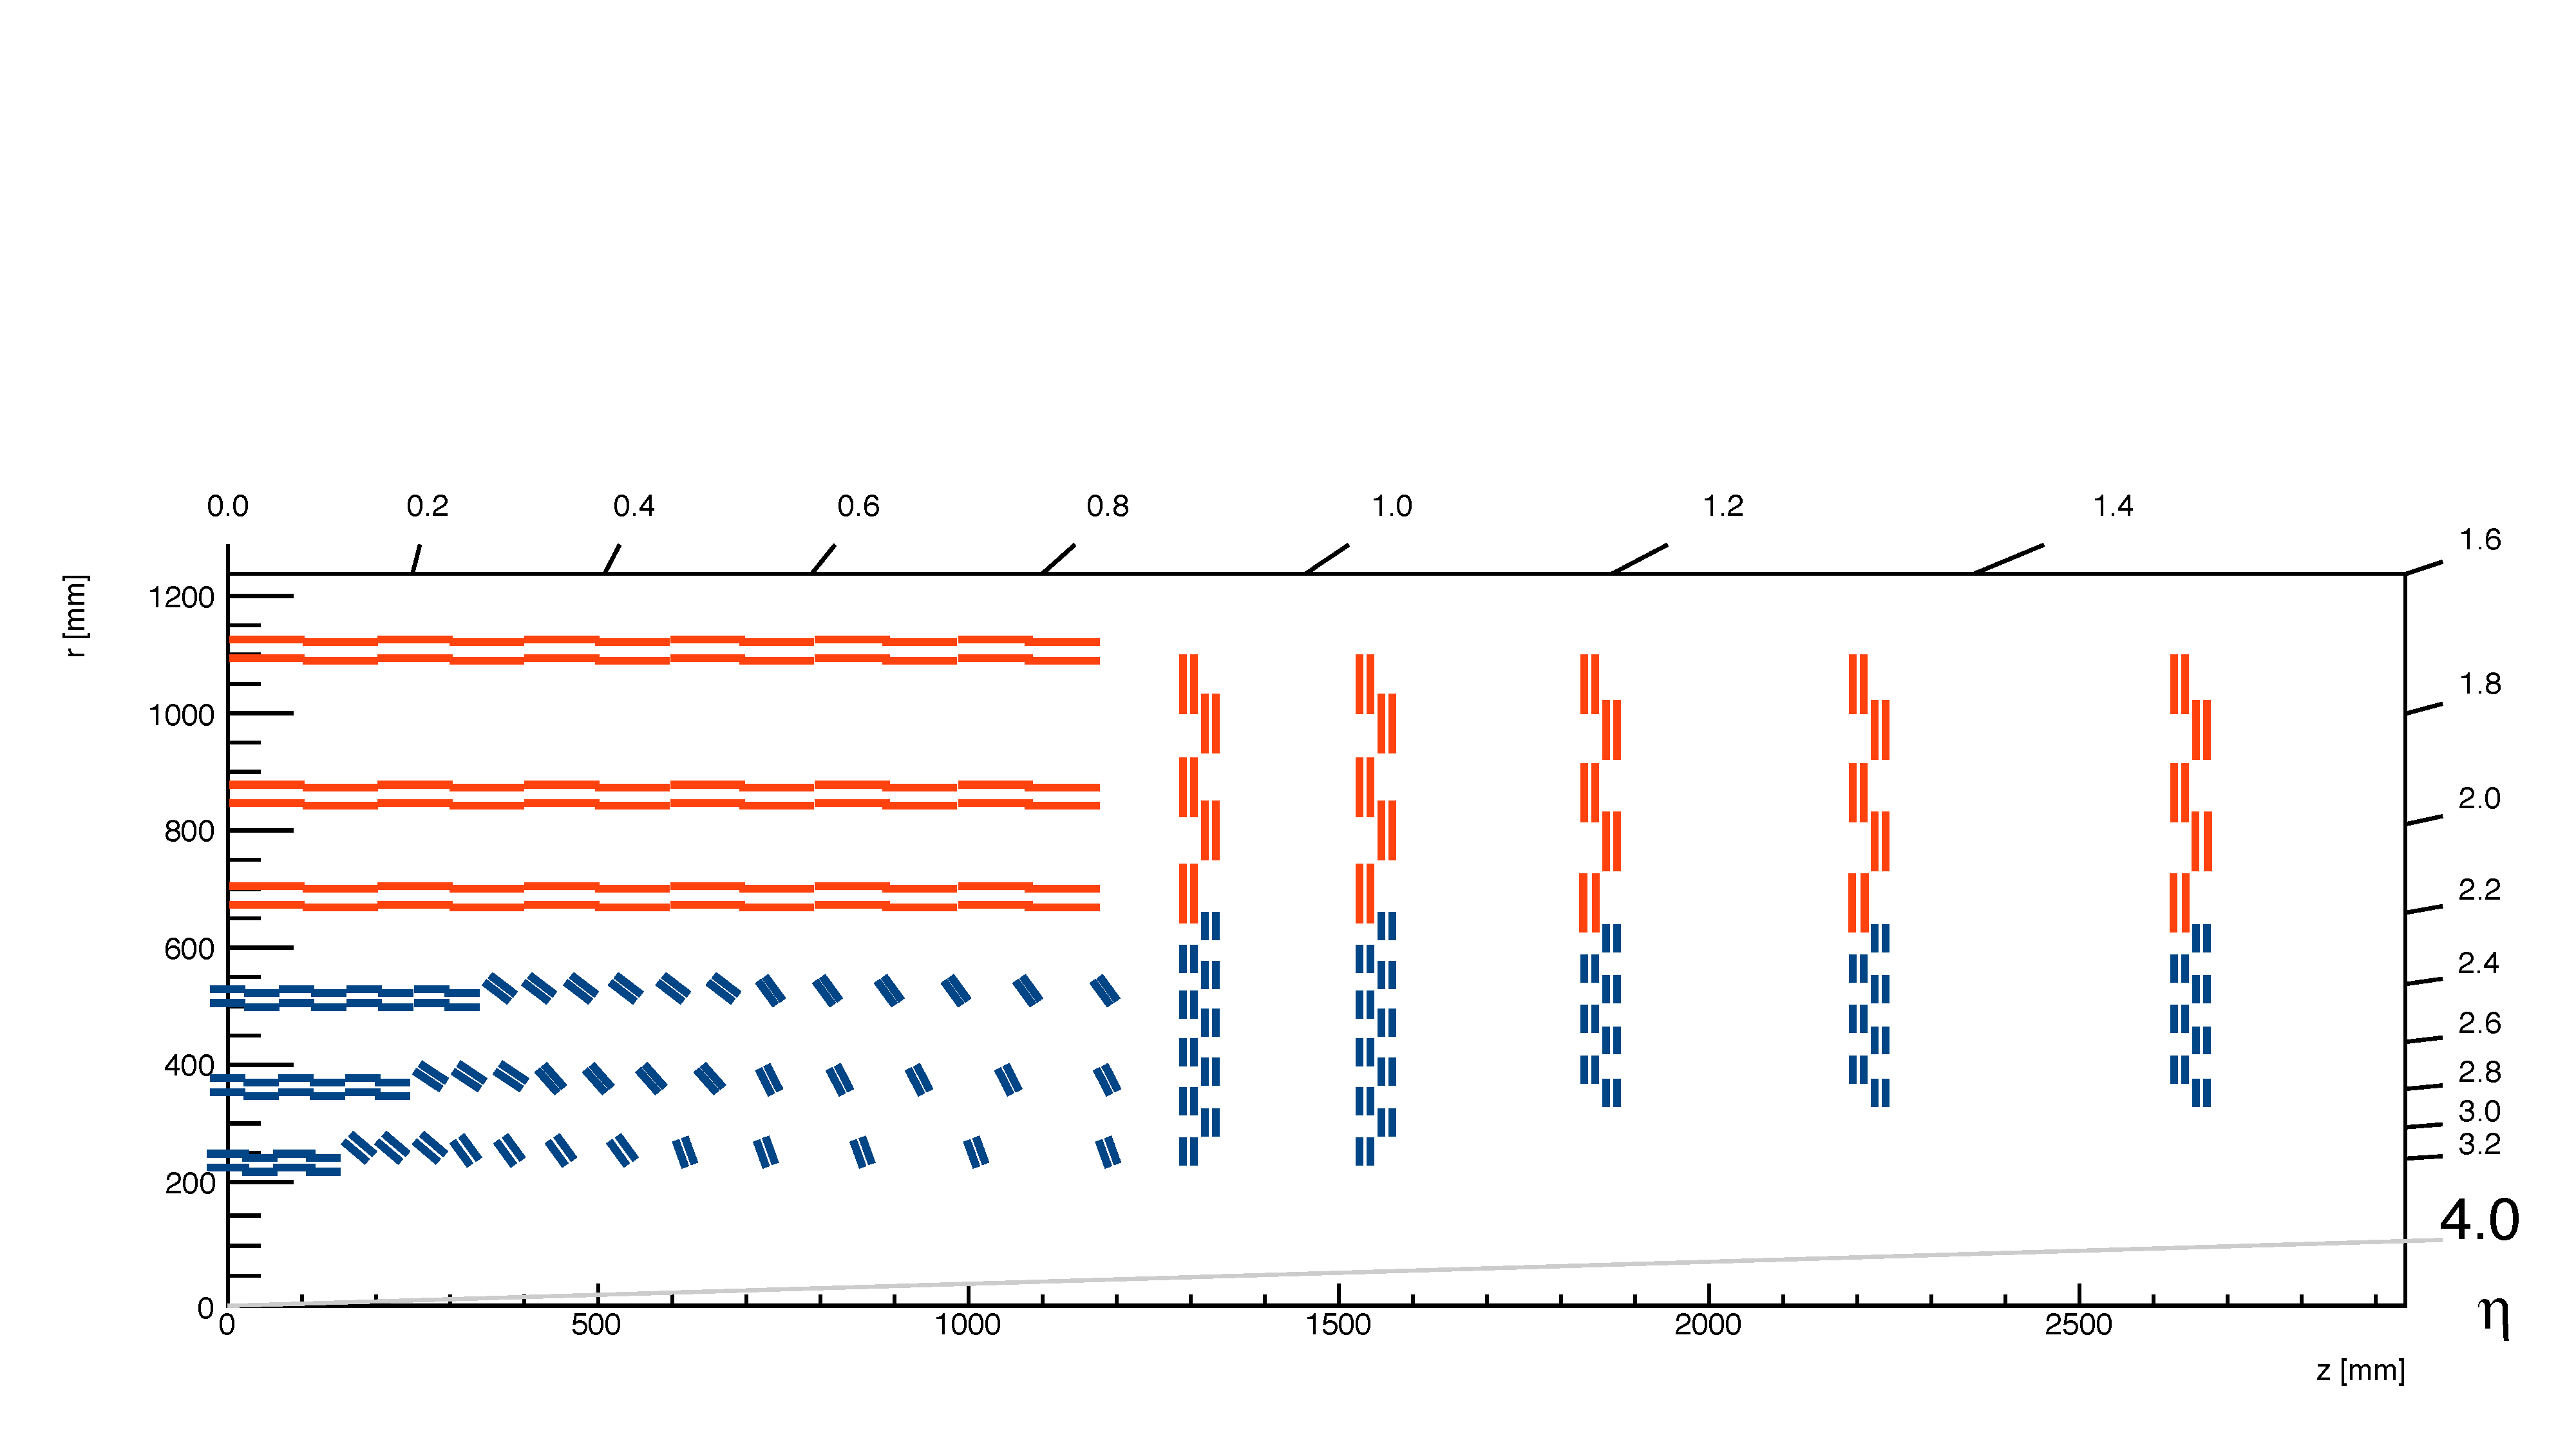
\includegraphics[width=0.8\textwidth,trim={1.1truecm 0truecm 1truecm 12truecm},clip]{figs/tk-upgrade/tiltedbarrelmap.pdf}
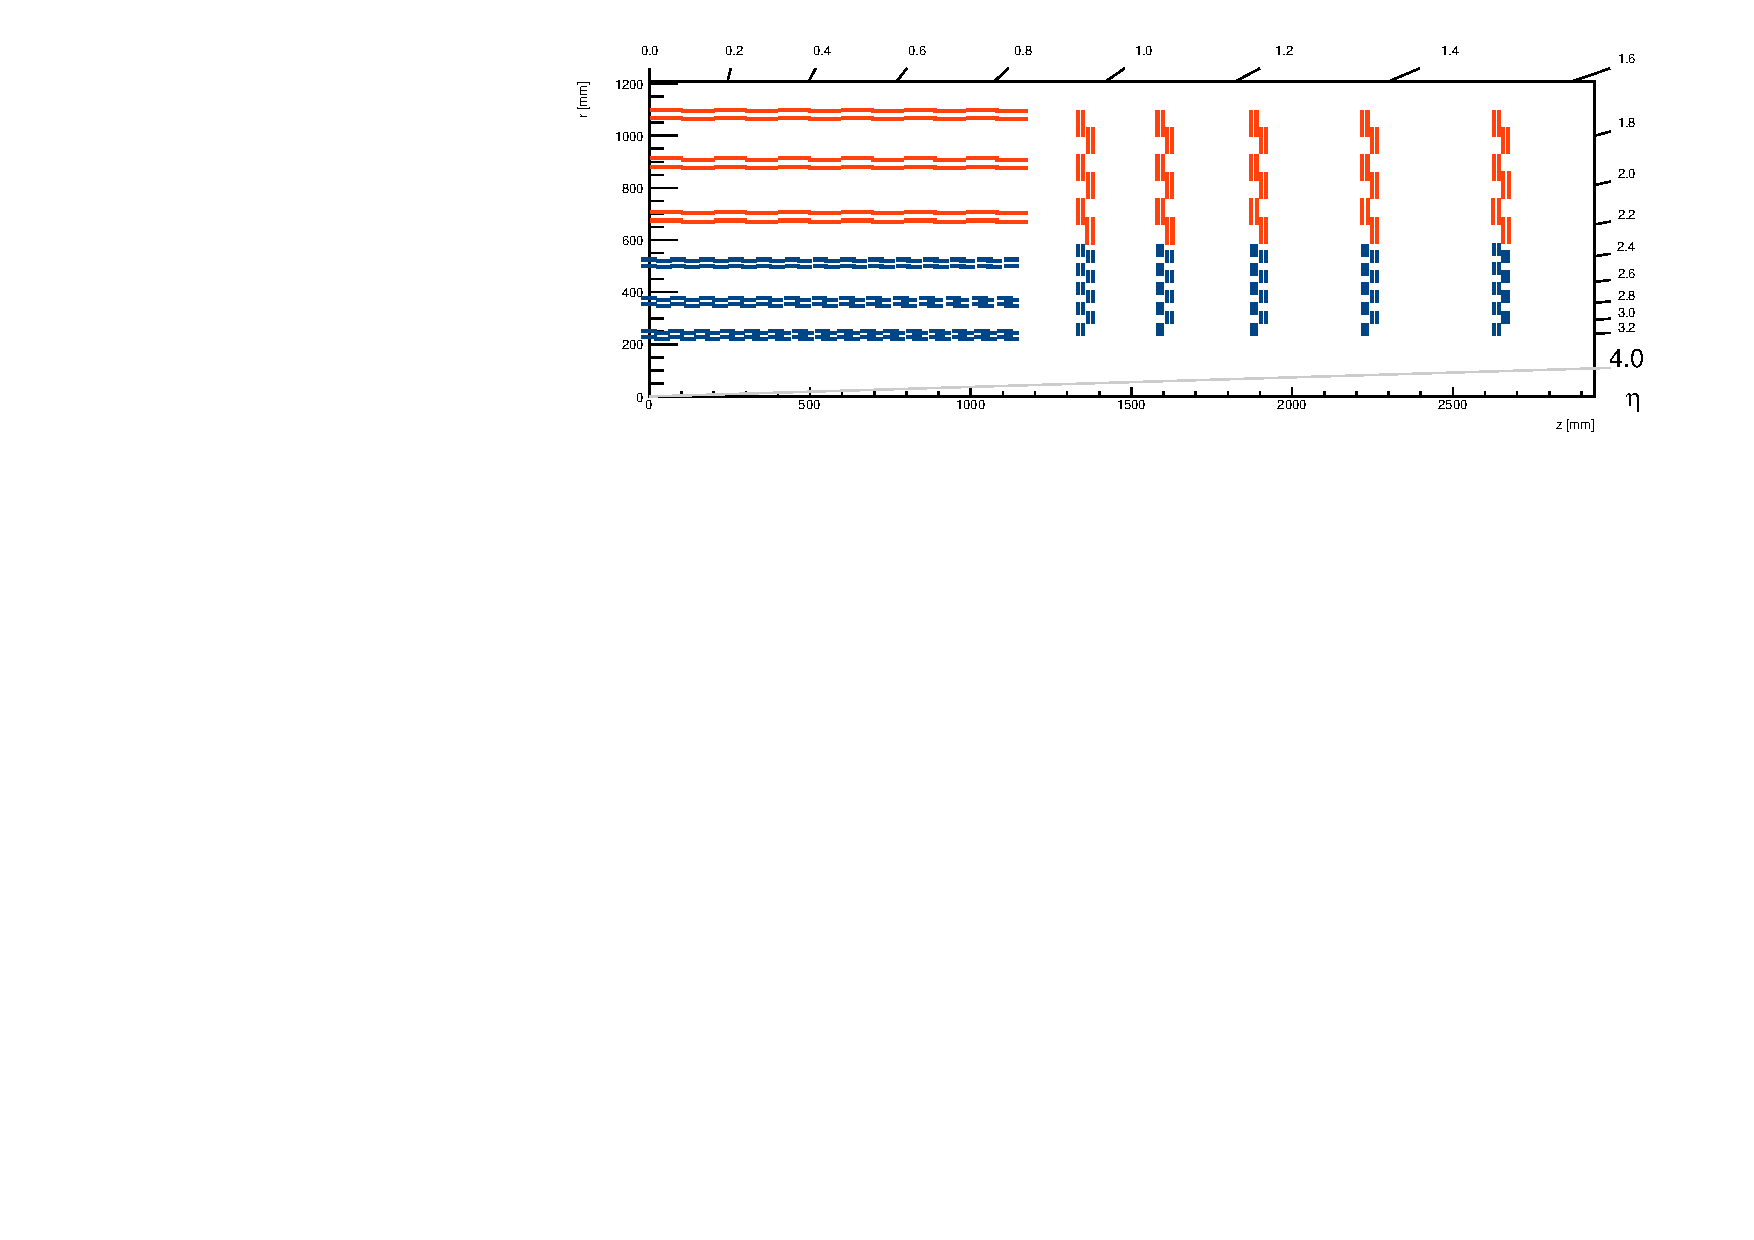
\includegraphics[width=0.8\textwidth,trim={0.7truecm 0truecm 1truecm 0truecm},clip]{figs/tk-upgrade/mersilayout.pdf}
\caption{One quadrant of the Phase-II Outer Tracker layout, showing the placement of the the PS (blue) and 2S (red) modules. The upper diagram shows the currently proposed \emph{tilted barrel} geometry~\cite{tiltedGeometry, P2TrackerTDR}, and the lower diagram shows an older proposal for the layout, known as the \emph{flat barrel} geometry \cite{CMS_Upgrade_TP}.}
\label{fig:trackerlayout}
\end{figure}

Out of the total L1 latency of 12.5\mus, $\approx 1\mus$ is required for generation, packaging and transmission of stubs from the tracker front-end electronics to the Data, Trigger and Control (DTC) system and $\approx 4\mus$ is available for the reconstruction of tracks from data arriving at the DTC, as shown in Fig.~\ref{fig:dataFlow}.
The rest of the available latency is allocated for the correlation of tracks with trigger primitives from the calorimeters and muon systems ($\approx 3.5\mus$), the propagation of the L1 decision to the front-end buffers ($1\mus$) and a safety margin ($3\mus$)~\cite{CMS_Upgrade_TP}.
Any Track Finder, which will take the stubs as input and output fully reconstructed tracks for the L1, proposed will be constrained by both being able to reconstruct tracks within the $4\mus$ latency constraint and how the detector is cabled to the DTC system.

\begin{figure}[tb]
\centering
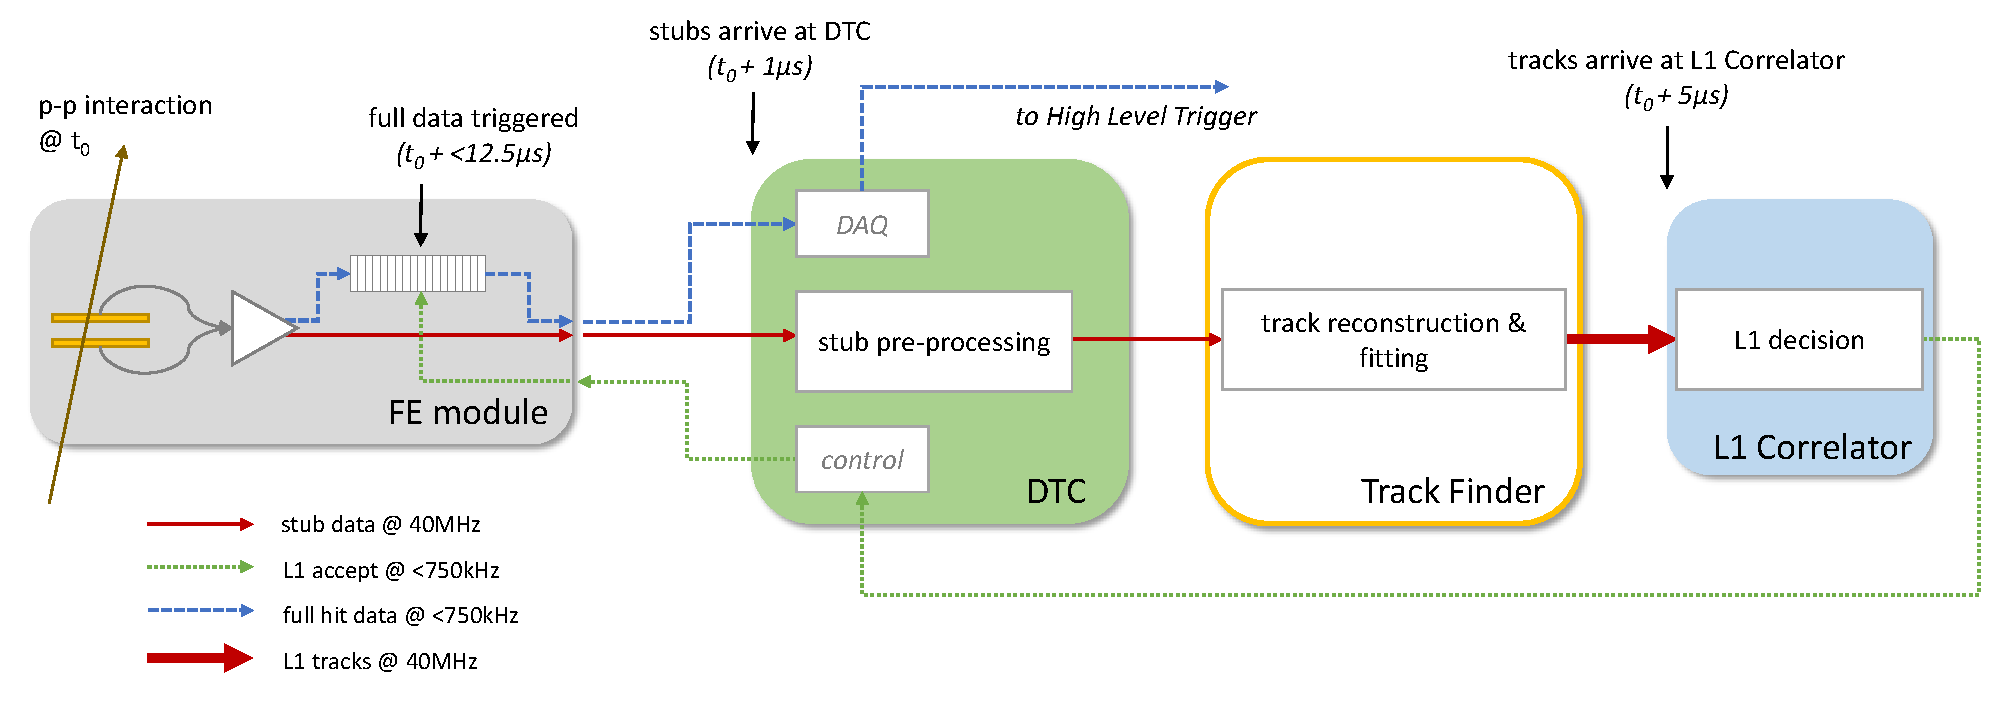
\includegraphics[width=\textwidth]{figs/tk-upgrade/dataflow.pdf}
% where an .eps filename suffix will be assumed under latex,
% and a .pdf suffix will be assumed for pdflatex; or what has been declared
% via \DeclareGraphicsExtensions.
\caption{Illustration of data-flow and latency requirements from \pt-modules through to the off-detector electronics dedicated to forming the L1 trigger decision.}
\label{fig:dataFlow}

Three different L1 track finders have been explored by the CMS Collaboration.
One uses Associative Memory (\emph{AM}) ASICs for track finding and FPGAs for track fitting, and the other two all-FPGA approaches, one using a Hough Transform (\emph{HT}) and the other a road search (\emph{tracklet}) algorithm to reconstruct tracks respectively.

Hardware demonstrators for each of the three proposed L1 track finder projects were constructed to prove the feasibility of each approach, which were reviewed in December 2016.
As all of the work discussed in this chapter was on the FPGA-based \HT approach, more detailed descriptions and results of both the AM and tracklet projects' approaches are not discussed here, but are given in~\cite{AM,P2TrackerTDR} and~\cite{tracklet,P2TrackerTDR} respectively.

At the time of the review, the then proposed \emph{flat barrel} geometry~\cite{CMS_Upgrade_TP} was used for all the studies undertaken, as depicted in the lower diagram in Fig.~\ref{fig:trackerlayout}.
Unless stated otherwise, the results discussed below use the old \emph{flat barrel} geometry instead of the currently proposed layout.

\section{An FPGA Based Track Finding Architecture and Processor}
\subsection{The Track Finding Architecture}

The proposed FPGA-based Hough Transform Track Finder is a fully time-multiplexed architecture, where parallel nodes each process a single event from multiple sources.
This allows for a scalable, flexible and redundant design as it allows the track finder to:
\begin{itemize}
\item be composed of identical processors which are fully pipelined (no sideways connections), thus allowing demonstration of the final system which a single Track Finding Processor (TFP).
\item make use of spare TFPs for online recovery in case of failure (which would be for a lost bunch crossing in N rather than a lost physical region) or parasitic testing of new algorithms during LHC runtime.
\end{itemize} 

At the time of the December 2016 review, it was assumed that the DTC system would be arranged such that it forms octants (\ie 45\,degree $\varphi$-sector) of the Outer Tracker, referred to here as \emph{detector octants}, which are non-uniform as the tracker geometry does not have an exact eight-fold symmetry.
By treating the DTC system as the first layer 

\subsection{The Track Finding Processor}
%The Track Finding Processor (TFP) described is based on a time-multiplexed approach. The outer tracking detector is split into eight $\phi$ octants, referred to as \textit{detector octants}, where $\phi$ is the azimuthal angle of the track. Each \textit{processing octant}, offset from the detector octant by 22.5 degrees in $\phi$ in order to handle data duplication across hardware boundaries, receives data from the Data, Trigger and Control (DTC) system. The DTC reads out each detector octant, unpacks and converts the stubs to a global coordinate system, and transmission to one or two processing octants, or if consistent with both, duplicates the stub into both octants. 
%
%Data consistent with each processing octant is sent out on separate links and processed by \textit{N} identical TFPs, negating the need for any data sharing downstream within or after the track finding process. This has the advantages of demonstrating a final system with one TFP which is easily scalable, allows for spare TFPs for online recovery in case of failure or online testing of new algorithms and allows each TFP to operate independently, thus reducing the requirements on system wide synchronisation.
%
%As the system is based on a time-multiplexed approach, each TFP processes only one event in \textit{N}. For our demonstrator system N was chosen to be thirty six, based on the currently available electronics and input/output links. 

%%tf-arch
The TFP (Fig.~\ref{fig:TFP}) consists of four self-contained components:
\begin{itemize}
\item {\bf Geometric Processor (GP)} - responsible for pre-processing the stubs from the DTC.
\item {\bf Hough Transform (HT)} - a highly panellised initial coarse track finding.
\item {\bf Kalman Filter (KF)} - cleans tracks, precisely fits helix parameters and removes fake tracks.
\item {\bf Duplicate Removal (DR)} - a final pass filter that uses the precise fit information to remove duplicate tracks generated by the \HT.
\end{itemize}

\begin{figure}[!h]
\centering
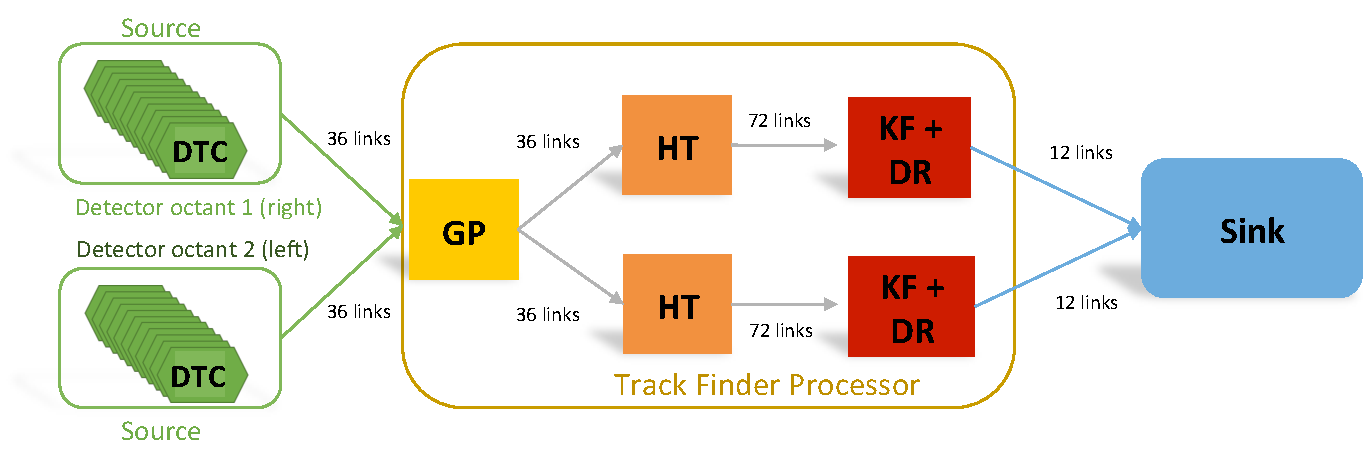
\includegraphics[width=0.78\textwidth]{figs/demoslice/demoslice1.pdf}
% where an .eps filename suffix will be assumed under latex,
% and a .pdf suffix will be assumed for pdflatex; or what has been declared
% via \DeclareGraphicsExtensions.
\caption{The four self-contained logical components of the Track Finding Processor, where each block represents a single FPGA. The two FPGAs for the two detector octant sources and the sink FPGA and the optical links between all components are also shown.}
\label{fig:TFP}
\end{figure}

A more complete description of the demonstrator system and all of the results achieved with up to the December 2016 review are described are given here~\cite{TMTT_JINST}.
\editComment{Relocate this sentence}

\subsubsection{Geometric Processor}
Each GP performs two tasks, firstly the conversion of the 48-bit DTC stubs into a 64-bit format extended format that is used to reduce the HT processing load and the assignment of stubs to thirty six sub-sectors, two sub-sectors in $\phi$ and eighteen in $\eta$ (where $\eta$ is the pseudo-rapidity). 
This division of the processing octants simplifies the task of the downstream logic required, allowing the track finding to be carried out independently and in parallel within each sub-sector. 
The relatively fine $\eta$ binning ensures that any track found by the \rphi HT is consistent in the \rz plane. Stubs compatible with more than one sub-sector, usually due to track curvature in $\phi$ are duplicated. 
The routing of stubs to sub-sectors occurs in three stages: a rough $\eta$ sorting into six bins, a fine $\eta$ sorting into three bins and a $\phi$ sorting into two bins. 
Each block in this router is highly reconfigurable and can easily be adapted to any alternative sub-sector definition.

\subsubsection{Hough Transform}
The Hough Transform algorithm is a widely used means of detecting geometric features in digital image processing \cite{HT}. 
It is used to find primary charged particles with \pT > 3\GeV in the \rphi plane. 
Within the tracking volume, permeated by a homogeneous 3.8T magnetic field ($B$), a radius of curvature ($R$) can be described as a function of its\pT and charge $q$:

\begin{equation}
R = \frac{\pt}{0.003\,qB} \;.
\label{eq:R}
\end{equation}

Assuming, to first order, that $R$ is constant, by neglecting energy losses such as through multiple scattering, and that only primary tracks from or near the primary interaction point are considered (other such tracks are not typically relevant to the L1 trigger), a stub with coordinates ($r$,$\varphi$) is related to $R$ by:

\begin{equation}
\frac r{2\,R} = \sin\left(\varphi-\phi\right)
\label{eq:stub_R}
\end{equation}

where $\phi$ is the angle of the track in the transverse plane at the origin \cite{markthesis}. 
For large \pT (> 3\GeV) and thus large $R$, the small angle approximation can be used. Combining Eq.~\ref{eq:R} and Eq.~\ref{eq:stub_R}, one produces the key formula showing the transformation from stub positions to straight lines in the track parameter plane (Hough-space):

\begin{equation}
\phi = \varphi - \frac{0.0015\,qB}{\pt}\cdot r \;.
\label{eq:localHT}
\end{equation}

The point of intersection of these lines in Hough-space would therefore correspond to a circle in the \rphi plane which is consistent with the primary interaction point and all stubs involved.

As the line gradients in Hough-space is given by the radius of the stubs, they will always be positive, the stub radius is transformed to $r_{58} = r - 58cm$ in order to utilise a larger phase space, which leads to fewer \textit{fake} (in that the found track does not match to a simulated particle) and duplicated tracks.

Given that $R$ for the lowest \pT track (3\GeV) to be considered is greater than the outer radius of the tracking detector ($r$ = 1.2m), all relevant particles are expected to traverse through at least six barrel layers or endcap disks. 
The threshold for the identification of a track candidate however, is set at a minimum of five detector layers or disk in order to allow for detector or readout inefficiencies. 
This threshold can be further reduced to four layers to account for the reduced geometric coverage between $0.89 < \eta < 1.16$ or for dead detector layers or disks.

\paragraph{Implementation}
A two stage fully pipelined design has been implemented in FPGA firmware, firstly the HT array is filled before the reading out of the HT track candidates. 

The \textit{Book Keeper} (Fig.~\ref{fig:implementationHT}) unpacks stub data from the input links and propagates stubs from one \textit{Bin} to the next each clock cycle, before the track candidate stubs are returned to the Book Keeper and transmitted downstream. 
Each Bin (Fig.~\ref{fig:implementationHT}) represents a $q/\pT$ column in the HT array. 
Using the left and right boundary results of the \HT calculation, it is determined if the stub crosses two $\phi$ rows and if so, it is duplicated and processed at the next available gap in the data stream. 
The stubs are sorted into the sixty four $\phi$ rows in the Track Builder's memory and if there are $\phi$ cells which meet the threshold requirement on the minimum number of hit layers/disks, the row is marked for readout. 
The \textit{Hand Shake} component is responsible for shifting the track candidate stubs from bin to bin until there are no further stubs, before enabling the reading out of the Track Builder.

\begin{figure}[!t]
\centering
\includegraphics[width=0.57\textwidth]{figs/tk-arch/ht/bookKeeper.pdf}
\includegraphics[width=0.37\textwidth]{figs/tk-arch/ht/bin.pdf}
% where an .eps filename suffix will be assumed under latex,
% and a .pdf suffix will be assumed for pdflatex; or what has been declared
% via \DeclareGraphicsExtensions.
\caption{Overview of a \textit{Book Keeper} (left) and a \textit{Bin}. Internal components are shown as boxes and data paths as lines, where arrows indicate the direction of data flow}
\label{fig:implementationHT}
\end{figure}

As the Book Keeper receives only one stub per clock cycle, thirty six arrays per octant are required to process the large number of stubs associated with each event at high pileup.
Each array (or Hough Segement) corresponds to one sub-sector from the GP, covering thirty two columns in \qpt and a sixty four row sub-range in $\varphi$.

A more detailed description of the firmware implementation of the \HT for the demonstrator system is discussed in \cite{IEEE} and \cite{TmttNote}.

\subsubsection{Kalman Filter}
Coarse \rphi helix parameters out of the \HT are used as the initial variables for track finding, with the segment assignment also providing a good seed value.
Given that in simulation over half the track candidates from by the HT are considered to be \textit{fake} or contain at least one stub associated with another particle, a Kalman Filter is used to both remove these incorrect stubs and reject fake tracks. 

In addition to the advantages of the Kalman filter for track reconstruction discussed by Fr{\"u}hwirth in \cite{Fruhwirth:1987fm}, the algorithm has several aspects making it suitable for FPGA implementation compared to global track fitting methods, namely the matrices:

\begin{itemize}
\item {are small.}
\item {are size independent of the number of measurements.}
\item {only involve the inversion of a small matrix.}
\end{itemize}

The initial estimate, or \textit{state}, of the track parameters and their uncertainties are updated by the KF iteratively applying stubs to update the state following the Kalman formalism, decreasing the uncertainty in the state. 
The relative uncertainties in the state and their associated measurements control parameter adjustment.
Missing layers can be skipped due to missing or incorrect stubs and multiple stubs on the same layer are each propagated and ranked, with up to the four best states being kept and presented to a final state selector.

As the final fit is always performed after a fixed period of time, there is no truncation in the traditional sense as all candidates will be read out, although events such as dense jets with many candidates and stubs per candidate will only be partially filtered.

A greater in-depth discussion of the mathematics and implementation of online track reconstruction using Kalman Filters on FPGAs in \cite{SSummers}.

\subsubsection{Duplicate Removal}
At the input to the DR, over half of the track candidates are unwanted duplicate tracks created by the HT.
Naively one would expect the need to compare pairs of tracks to see if they are the same as each other, but by understanding how the HT produces these duplicate tracks a more elegant and subtle DR algorithm can be used.
This approach is illustrated in Fig.~\ref{fig:DR}, where five stubs (blue lines in Hough Space) produces three candidates (green and yellow cells).
As all three candidates contain the same stubs, they will be fitted with identical helix parameters in the same cell (the yellow cell) regardless of the original HT cell.
The algorithm accepts only tracks whose fitted parameters are consistent to those that the HT found them in initially. There is however, a small subtlety, given that the algorithm eliminates unique tracks whose fitted parameters were not consistent, which results in the loss of a few percent of efficiency. 
By performing a second pass through the rejected tracks and rescuing those which are unique the lost efficiency can be recovered.

\begin{figure}[!h]
\centering
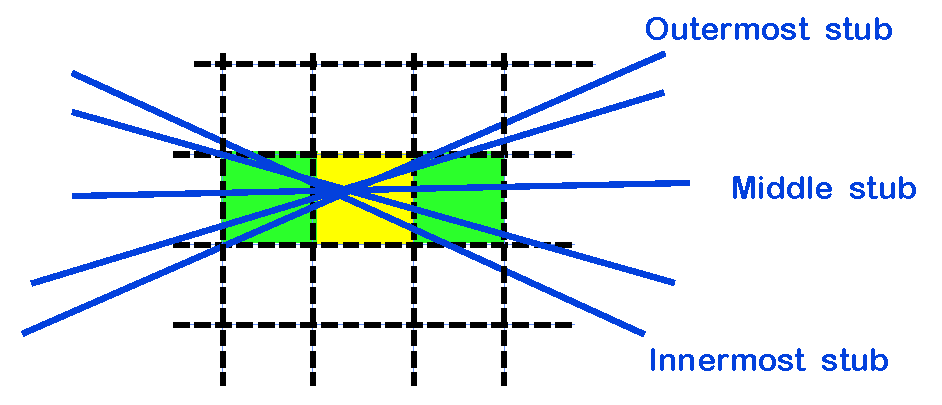
\includegraphics[width=0.80\textwidth]{figs/tk-arch/dr/A50_algo.pdf}
% where an .eps filename suffix will be assumed under latex,
% and a .pdf suffix will be assumed for pdflatex; or what has been declared
% via \DeclareGraphicsExtensions.
\caption{Illustration of how duplicates are formed by the \rphi \HT.}
\label{fig:DR}
\end{figure}

\paragraph{Implementation}
A minimum resource usage strategy has resulted in firmware that can be integrated in the same board as the KF.
Tracks which are consistent in both HT and KF space are marked in a matrix, which allows only one track per cell, are forwarded to the output.
Tracks which are not consistent and not yet in the matrix are kept in a FIFO until a certain time threshold is reached, then, if the tracks point to a still unmarked cell, they are marked in the matrix and forwarded to the output. 

Two matrices are used in an interleaving fashion as a complete reset is required before processing tracks from the following event.
Additionally, two FIFOs (one per matrix) are required to store the addresses that were marked and thus require to be cleared in the event, therefore resulting in there being always one active and one resetting matrix.

\section{Simulation Studies}
During the development of the TMTT demonstrator system both before and following the December 2016 review, the author was involved in a number of simulation studies, the more substantive of which are discussed below.

\subsection{Linear $\chi^{2}$ Track Fitter}
Whilst the Kalman Filter was used as a track fitter for the December 2016 hardware demonstrator, two alternative track fitting algorithms, a Seed Filter (SF) and Linear Regression (LR) fitter and Linearised $\chi^{2}$ fitter were explored.
The SF+LR works by removing stubs in a HT cell which are inconsistent with a straight line the \emph{r-z} plane before  two independent fits in the \emph{r-$\varphi$/r-z} planes with a linear regression technique are made, and is further discussed in~\cite{TMTT_FLP}.
The 

%%internal cuts, multiple iterations

%% limits of maths/LUTs/resources required

\subsection{Flexibility and Robustness of the System}
\subsubsection{2 GeV Tracking}
The flexibility to reconstruct tracks down to a lower \pT threshold of 2\GeV may be desirable if the trigger requirements demand it and the impact of this potential requirement on the proposed track-finder system was studied for the December 2016 demonstrator review.
This required modifying the GP and HT configuration parameters to ensure adequate duplication in $\varphi$ and increasing the number of the \qpt columns by 50\% to take into account the increased \pt range whilst maintaining the same precision, respectively.
The increased \qpt range consequently increases the FPGA resources required by 50\% and increases the output data rate from the \HT by a factor of 2.2.

Without any further modifications, there is a considerable degradation in the track reconstruction efficiency in the range $2 < \pt < 2.7$\GeVc, predominantly due to multiple scattering which results in stubs not always intersecting within a single \HT cell and thus failing to exceed the threshold criteria and generate track candidates.
%%% Causes - mainly multiple scattering, what else?
To mitigate against this issue, the precision of the \HT cells along \qpt and $\phi_{T}$ for the range $2 < \pt < 2.7$\GeVc was reduced by a factor of two and the internal \KF State Accumulator $\chi^2$ cuts for the range $2 < \pt < 2.7$ were optimised to reduce the number of duplicate and fake tracks as far as possible without impacting on the track reconstruction efficiency.
This variable precision \HT, which has been separately implemented in firmware, has been shown in simulation to recover some of this loss, as shown in Fig~\ref{fig:2GeVFlat}

\begin{figure}[tbp]
\centering

\includegraphics[width=0.8\textwidth,trim={1.1truecm 0truecm 1truecm 12truecm},clip]{CMS-bw-logo.pdf}

\includegraphics[width=0.8\textwidth,trim={0.7truecm 0truecm 1truecm 0truecm},clip]{CMS-bw-logo.pdf}
\caption{Images showing tracking efficiency in low pT range with no changes (upper), and with HT cell merging (right)}
\label{fig:2GeVFlat}
\end{figure}

%%% Discuss poorer tracking efficiency
%%% How to fix:
%%% - merging of low pT HT cells
%%% Causes - mainly multiple scattering, what else?
%%% - KF internal chi-squared cuts; would expect if MS was fully accounted for, then on average chi2/NDF = 1  everywhere. Show chi2/NDF vs eta plots?

Following the December 2016 demonstrator review, further progress was made in improving tracking down to 2\GeV.

%%% - additive constant of order (1 mrad)^{2}
%%% - additive constant / radius

Further improvements to the \HT, such as \pt dependent threshold criteria and optimisation of the \KF to such changes, should be able to 

\subsubsection{Alternative cabling schemes}
%% Motivation
Since the December 2016 review, an alternative tracker cabling scenario has been proposed where a nonant segmentation in $\varphi$ is used instead instead an octant segmentation.
Without any modifications to the system, the implication of an additional TFP per time slice required for the additional segment is the need for another 

%% Implications
%% Increase phi octants from 8 to 9, number of phi sectors from 16 to 18, num of Phi HT bins is 64->56
%% Each HT cell is thus larger in phi by a factor (8/9)*(64/56). 